\section{Simulation Analysis}
\label{sec:simulation}

\hspace{0,5cm} This section covers the audio amplifier circuit simulation using the Ngspice tool.
\par As asked in the lab assignment, a NPN transistor and a PNP transistor were used in gain stage and output stage respectively. The goal was to calculate the impedances ($Z_I$ and $Z_O$), the cut off frequencies (), the bandwidth (the difference between the cut off frequencies) and the total gain. Also the goal was to optimize these values.
\par It was also confirmed if the BJTs are on the F.A.R. (forward active region) by comparing $V_{CE}$ and $V_{BE}$ for NPN type and $V_{EC}$ and $V_{EB}$ for PNP type. The merit is also calculated in this section.
\par Later in this report, we will compare this results with the theoretical ones but for now we will just show them.

\par The Table~\ref{tab:ng2} and \ref{tab:ng3} shows the BJTs voltages and their F.A.R. confirmation.

\begin{table}[!ht]
  \centering
  \begin{tabular}{|l|r|}
    \hline    
    {\bf Name} & {\bf Value [A or V]} \\ \hline
    V(CE) & 2.78156\\ \hline
V(BE) & 0.70931\\ \hline
V(CE)>V(BE) & Yes\\ \hline

  \end{tabular}
  \caption{F.A.R. confirmation - BC547A (NPN type)}
  \label{tab:ng2}
\end{table}

\begin{table}[!ht]
  \centering
  \begin{tabular}{|l|r|}
    \hline    
    {\bf Name} & {\bf Value [A or V]} \\ \hline
    V(EC) & 4.49605\\ \hline
V(EB) & 0.817257\\ \hline
V(EC)>V(EB) & Yes\\ \hline

  \end{tabular}
  \caption{F.A.R. confirmation - BC557A (PNP type)}
  \label{tab:ng3}
\end{table}

\par After the OP analysis where the currents branches and nodal voltages were computed, in the next table it is presented the values asked: voltage gain, lower and upper cut off frequency and the bandwidth. It was used the .meas function.

\begin{table}[!ht]
  \centering
  \begin{tabular}{|l|r|}
    \hline    
    {\bf Name} & {\bf Value [A or V]} \\ \hline
    V_Gain&37.9181\\ \hline
Bandwidth&1.55393E+06\\ \hline
CO_Freq& 8793.49\\ \hline

  \end{tabular}
  \caption{Ngspice simulation results}
  \label{tab:ng4}
\end{table}

\par EFFECT OF THE COUPLING'S CAPACITOR: To fully analyse this circuit it is fundamental to understand the Coupling's Capacitor behaviour. The main effect of the Coupling's Capacitor is to block the DC signals of the Audio In source. When the capacitance is increased, the cut off frequency is anticipated leading to a larger bandwidth. This results in the capacitor blocking some lower frequencies influencing directly in the bandwidth.

\par EFFECT OF THE BYPASS CAPACITOR: As studied in classes, the Re stabilizes the effect of the temperature in the DC voltage. On the other hand, this accomplishment has a negativa effect on the gain stage of the audio amplifier, it lowers the gain voltage. By placing the capacitor in parallel with the resistor Re, this resistor becames short for high frequencies (impedance of the capacitor is $\frac{1}{j\omega L}$, having an extreme importance in maximazing the gain for medium and high frequencies.

\par EFFECT OF THE $R_c$: It is also relevant to analyse the influence of $R_c$ on the total gain stage of the circuit. The gain increases with $R_c$ as was already predicted in Section~\ref{sec:analysis}.

\par In the following graphics it can be seen how the effect of the previous components and how the the input voltage and output voltage varies with the frequency.

\begin{figure}[ht!] \centering
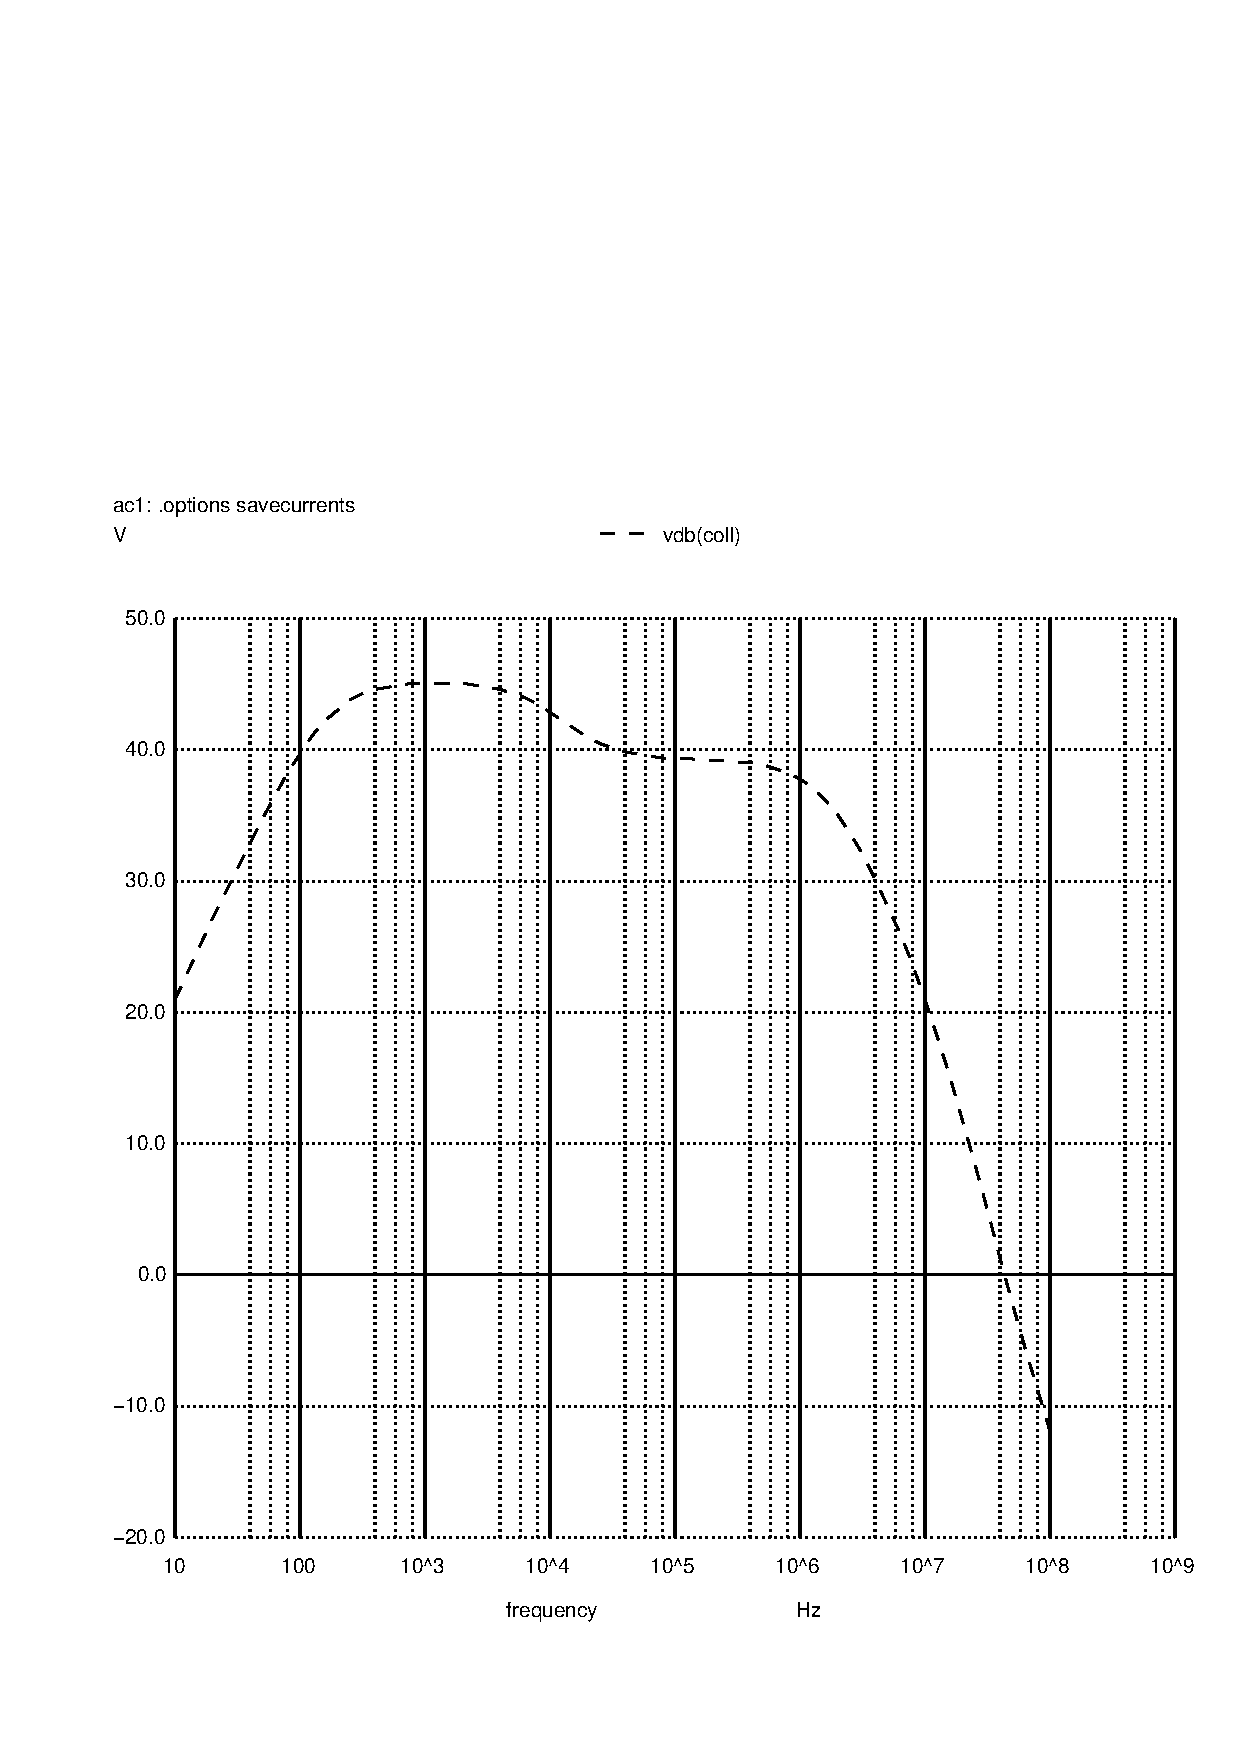
\includegraphics[width=0.5\linewidth]{../sim/vo1f.pdf}
\caption{Input Voltage} 
\label{fig:sim1}
\end{figure}

\begin{figure}[ht!] \centering
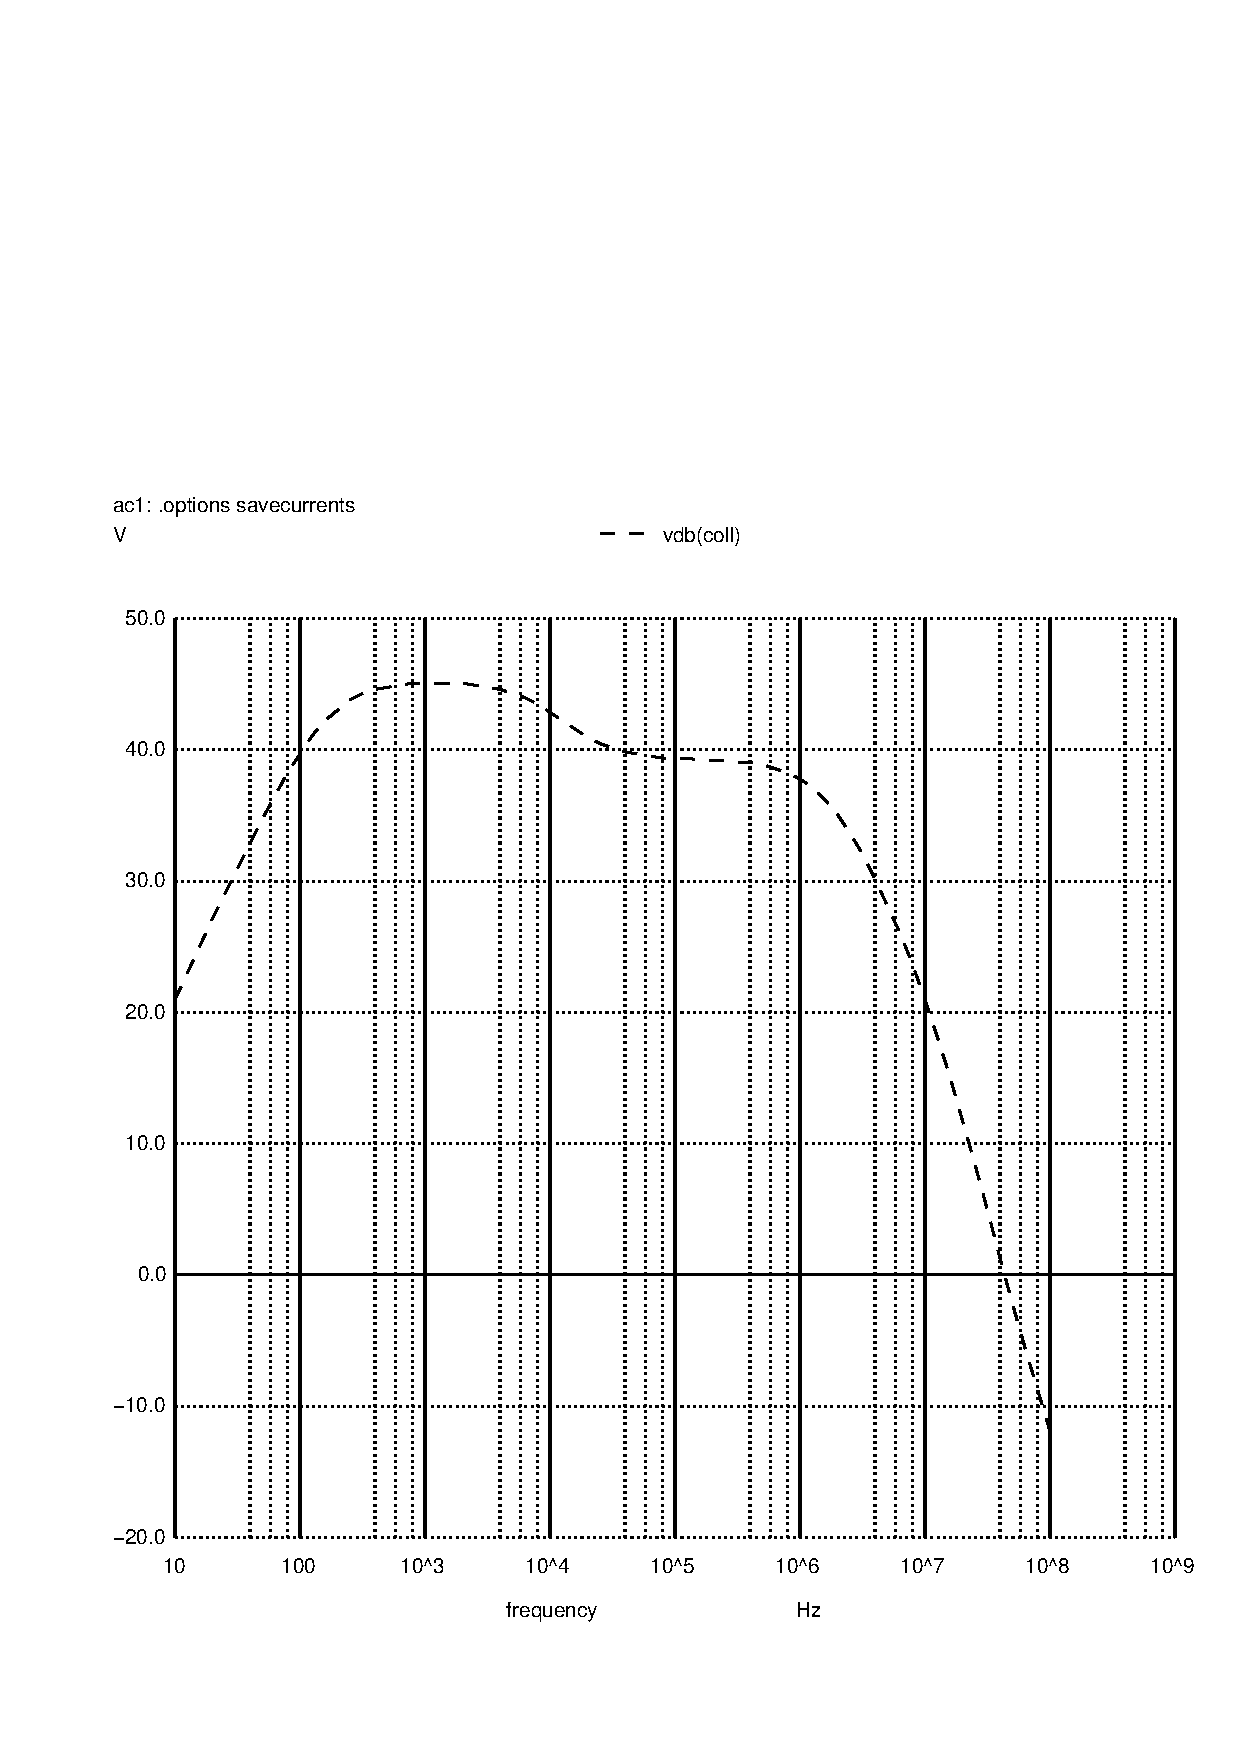
\includegraphics[width=0.5\linewidth]{../sim/vo2f.pdf}
\caption{Output Voltage} 
\label{fig:sim2}
\end{figure}

\par To guarantee a high compatability between Audio In and the speakers is important to simulate the input and outpu impedances. To have a the a similar voltage in node In2 and Vin it is necessary a high resistance value. Regarding the output impedance, it must be the lowest possible, in order to have the maxime output voltage.

\begin{table}[!ht]
  \centering
  \begin{tabular}{|l|r|}
    \hline    
    {\bf Name} & {\bf Value [A or V]} \\ \hline
    Zin & -548.062 + 82.7641 j\\ \hline

  \end{tabular}
  \caption{Impedance values}
  \label{tab:ng5}
\end{table}

\par The merit obtained by the group is presentend in the following table. It can be consider tha the results were good.

\begin{table}[!ht]
  \centering
  \begin{tabular}{|l|r|}
    \hline    
    {\bf Name} & {\bf Value [A or V]} \\ \hline
    Cost & 123.208\\ \hline
merit & 54.3849\\ \hline

  \end{tabular}
  \caption{Cost and merit results}
  \label{tab:ngs1}
\end{table}


